\section{Battery State of Charge\label{sec:5_battery}}
BEBs must also maintain their state of charge above a minimum threshold, denoted $h_{\text{min}}$. Let $h_{ij+1}$ be the state of charge for bus $i$ at the beginning of stop $j$. Each bus has an initial state of charge defined by $h_{i0}$ as shown in figure \ref{fig:hPlacement}. 
\begin{figure*}
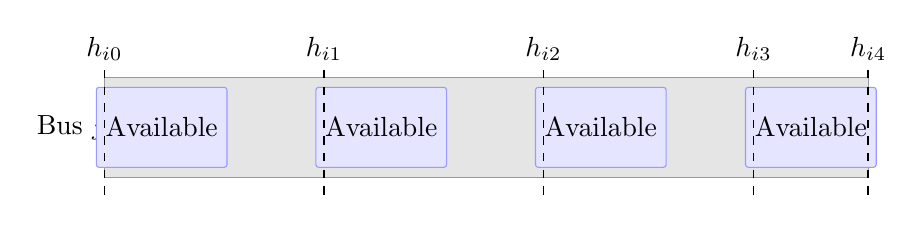
\begin{tikzpicture}
\node[rectangle, draw=black!40, fill=black!10, minimum width=0.8\textwidth, minimum height=0.5in](charger1Box) at (0.5\textwidth,1){};
	\node(bus1BoxLabel) at (0.065\textwidth, 1){Bus $j$}; 
	\node[rectangle, draw=blue!40, fill=blue!10, minimum width=0.12\textwidth, minimum height=0.4in, rounded corners=1pt] at (0.16\textwidth,1){Available};
	\node[rectangle, draw=blue!40, fill=blue!10, minimum width=0.12\textwidth, minimum height=0.4in, rounded corners=1pt] at (0.39\textwidth,1){Available};
	\node[rectangle, draw=blue!40, fill=blue!10, minimum width=0.12\textwidth, minimum height=0.4in, rounded corners=1pt] at (0.62\textwidth,1){Available};
	\node[rectangle, draw=blue!40, fill=blue!10, minimum width=0.12\textwidth, minimum height=0.4in, rounded corners=1pt] at (0.84\textwidth,1){Available};

	\node(h0High) at (0.1\textwidth,2){$h_{i0}$};
	\node(h0Low) at (0.1\textwidth,0.05){};
	\draw[dashed, line width=0.5pt] (h0High) -- (h0Low.center);

	\node(h1High) at (0.33\textwidth,2){$h_{i1}$};
	\node(h1Low) at (0.33\textwidth,0.05){};
	\draw[dashed, line width=0.5pt] (h1High) -- (h1Low.center);

	\node(h0High) at (0.56\textwidth,2){$h_{i2}$};
	\node(h0Low) at (0.56\textwidth,0.05){};
	\draw[dashed, line width=0.5pt] (h0High) -- (h0Low.center);

	\node(h0High) at (0.78\textwidth,2){$h_{i3}$};
	\node(h0Low) at (0.78\textwidth,0.05){};
	\draw[dashed, line width=0.5pt] (h0High) -- (h0Low.center);

	\node(h0High) at (0.9\textwidth,2){$h_{i4}$};
	\node(h0Low) at (0.9\textwidth,0.05){};
	\draw[dashed, line width=0.5pt] (h0High) -- (h0Low.center);
\end{tikzpicture}
\caption{State of Charge Variables}
\label{fig:hPlacement}
\end{figure*}

This can be constrained as
\begin{equation}\label{eqn:initialSoc0}
	h_{i0} = \eta_{i} \ \forall i.
\end{equation}
where $\eta_{i}$ is the initial state of charge for bus $i$.
Equation \ref{eqn:initialSoc0} can be expressed in standard form such that
\begin{equation} \begin{aligned}
	\begin{bmatrix}0 & 0 & \hdots & 0 & 1_i& 0 \end{bmatrix}\mathbf{y} &= \eta_i \ \forall i \\
		\tilde{A}_1\mathbf{y} &= \tilde{\mathbf{b}}_1
\end{aligned} \end{equation}
\begin{figure*}
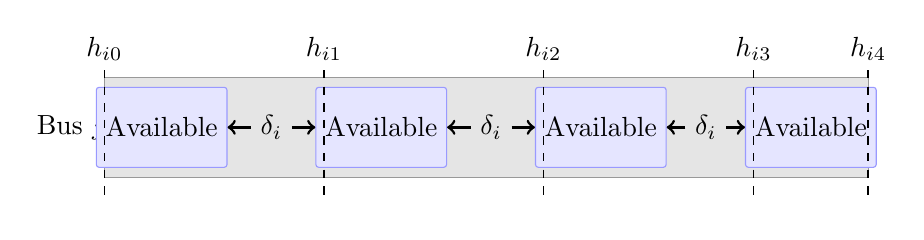
\begin{tikzpicture}
\node[rectangle, draw=black!40, fill=black!10, minimum width=0.8\textwidth, minimum height=0.5in](charger1Box) at (0.5\textwidth,1){};
	\node(bus1BoxLabel) at (0.065\textwidth, 1){Bus $j$}; 
	\node[rectangle, draw=blue!40, fill=blue!10, minimum width=0.12\textwidth, minimum height=0.4in, rounded corners=1pt](avail1) at (0.16\textwidth,1){Available};
	\node[rectangle, draw=blue!40, fill=blue!10, minimum width=0.12\textwidth, minimum height=0.4in, rounded corners=1pt](avail2) at (0.39\textwidth,1){Available};
	\node[rectangle, draw=blue!40, fill=blue!10, minimum width=0.12\textwidth, minimum height=0.4in, rounded corners=1pt](avail3) at (0.62\textwidth,1){Available};
	\node[rectangle, draw=blue!40, fill=blue!10, minimum width=0.12\textwidth, minimum height=0.4in, rounded corners=1pt](avail4) at (0.84\textwidth,1){Available};

	\node(h0High) at (0.1\textwidth,2){$h_{i0}$};
	\node(h0Low) at (0.1\textwidth,0.05){};
	\draw[dashed, line width=0.5pt] (h0High) -- (h0Low.center);

	\node(h1High) at (0.33\textwidth,2){$h_{i1}$};
	\node(h1Low) at (0.33\textwidth,0.05){};
	\draw[dashed, line width=0.5pt] (h1High) -- (h1Low.center);

	\node(h0High) at (0.56\textwidth,2){$h_{i2}$};
	\node(h0Low) at (0.56\textwidth,0.05){};
	\draw[dashed, line width=0.5pt] (h0High) -- (h0Low.center);

	\node(h0High) at (0.78\textwidth,2){$h_{i3}$};
	\node(h0Low) at (0.78\textwidth,0.05){};
	\draw[dashed, line width=0.5pt] (h0High) -- (h0Low.center);

	\node(h0High) at (0.9\textwidth,2){$h_{i4}$};
	\node(h0Low) at (0.9\textwidth,0.05){};
	\draw[dashed, line width=0.5pt] (h0High) -- (h0Low.center);

	\node(delta1) at (0.275\textwidth,1){$\delta_i$};
	\draw[->, line width=1pt] (delta1.west) -- (avail1.east);
	\draw[->, line width=1pt] (delta1.east) -- (avail2.west);
	\node(delta2) at (0.505\textwidth,1){$\delta_i$}; 
	\draw[->, line width=1pt] (delta2.west) -- (avail2.east);
	\draw[->, line width=1pt] (delta2.east) -- (avail3.west);
	\node(delta3) at (0.73\textwidth,1){$\delta_i$}; 
	\draw[->, line width=1pt] (delta3.west) -- (avail3.east);
	\draw[->, line width=1pt] (delta3.east) -- (avail4.west);
\end{tikzpicture}
\caption{Placement for $\delta_i$}
\label{fig:hPlacement}
\end{figure*}

\par The transition from $h_{ij}$ to $h_{ij+1}$ is computed as the sum of battery effects due to charging and discharging. The discharge from operating bus $i$ over one route loop is denoted $\delta_i$. The increase in battery state of charge follows a linear charge model\cite{rong_coordinated_2016} such that the increase is equal to the energy rate, denoted $p$, times the time spent charging, denoted $\Delta_{\text{sc}}$.
The total change from $h_{ij}$ to $h_{ij+1}$ can be expressed as
\begin{equation}
	h_{ij+1} = h_{ij} + \Delta T\cdot p - \delta_i.
\end{equation}
The value for $\Delta T$ can also be expressed in terms of the difference between $a_{ij}$ and $d_{ij}$ such that
\begin{equation}\label{eqn:socDynamic1}\begin{aligned}
	h_{ij+1} &= h_{ij} + p\cdot \left ( s_{ij} - c_{ij} \right ) - \delta_i\\
	h_{ij+1} - h_{ij} - ps_{ij} + pc_{ij} &= -\delta_i\\
	\begin{bmatrix} 1 & -1 & -p & p\end{bmatrix} \begin{bmatrix}h_{ij+1} \\ h_{ij} \\ s_{ij} \\ c_{ij} \end{bmatrix} &= -\delta_i \ \forall i,j
\end{aligned}\end{equation}
The constraints for each $i,j$ outlined in equation \ref{eqn:socDynamic1} can be vertically concatenated to form
\begin{equation}\label{eqn:socDynamic3} \begin{aligned}
	A_{ij}\mathbf{y} &= \mathbf{b}_{ij} \ \forall i,j \\
	\tilde{A}_2\mathbf{y} &= \tilde{\mathbf{b}}_2
\end{aligned} \end{equation}
Now that the state of charge is defined, the final constraint ensures that the minimum battery state of charge is kept above the minimum threshold, $h_{\text{min}}$. These constraints are given as
\begin{equation}
	-h_{ij} \le -h_{\text{min}} \ \forall i,j
\end{equation}
or 
\begin{equation} \begin{aligned}
	\begin{bmatrix}0 & \hdots & 0 & -1_{h} & 0 & \hdots & 0\end{bmatrix} \mathbf{y} &\le \mathbf{1}\cdot h_{\text{min}}\\ 
		A_5\mathbf{y} &\le \mathbf{b}_5
\end{aligned} \end{equation}
\par The final constraint has to do with the assumption that we are modeling one day and want to repeat the cost to predict the expected cost over a month. In order to do this, the state of charge at the end of the day must equal the state of charge at the beginning. Let $h_{i,\text{end}}$ be the final daily state of charge for bus $i$. This is constrained to be the same as the beginning state of charge as
\begin{equation} \label{eqn:hEqual1} \begin{aligned}
	h_{i0} &= h_{i,\text{end}} \ \forall i \\
	h_{i0} - h_{i,\text{end}} &= 0 \ \forall i.  
\end{aligned} \end{equation}
However, because equality for two continuous variables is computationally demanding, the constraint in equation \ref{eqn:hEqual1} can also be expressed as 
\begin{equation} \begin{aligned}
	h_{i0} - h_{i,\text{end}} \le 0.
\end{aligned} \end{equation}
Because the final state of charge is dependent on the amount of power used to charge, and power/energy use is penalized (see section \ref{sec:objective}), the optimization process will force the final state of charge down until is nearly equal to the initial.
TODO:
\begin{enumerate}
	\item Add section that talks about constraints to keep the battery SOC below the maximum SOC
\end{enumerate}
